% !TEX root = main-crime.tex

\section{Overview}
\label{sec:overview}
The crime data collected in Chicago has detailed information about the time and location (i.e., latitude and longitude) of crime and the types of crime. In our problem, the term crime count refers to number of crime incidents in a region (i.e., community area) in a year. The \emph{community area} is used as our geographical unit of study, since it is well-defined,  historically recognized and stable over time~\cite{wiki-ca}. In total, there are 77 community areas in Chicago.  Crime rate is the crime count normalized by the population in a region. We use vector $\vec{y} = [y_1, y_2, \ldots, y_n]$ to denote the crime rates in regions. The crime rate inference problem is to estimate the crime rate in one region using the crime rate of other regions in the same year by considering the features of regions and correlations between regions. 


The crime data of Chicago are obtained from the City of Chicago data portal~\cite{crime-data}. Chicago is the city with most complete crime data that are made public online. The crime dataset contains the incident date, location (strict name and GPS coordinates), and primary type from year 2001 to 2015. In total there are \num{5856414} recorded crime incidents over 15 years, which is an average \num{390417} crimes incidents per year. We visualize the crime normalized by population in Figure~\ref{fig:crime-ca}, from which we can see that the downtown area has the highest crime rate.

\begin{figure}[t]
\centering
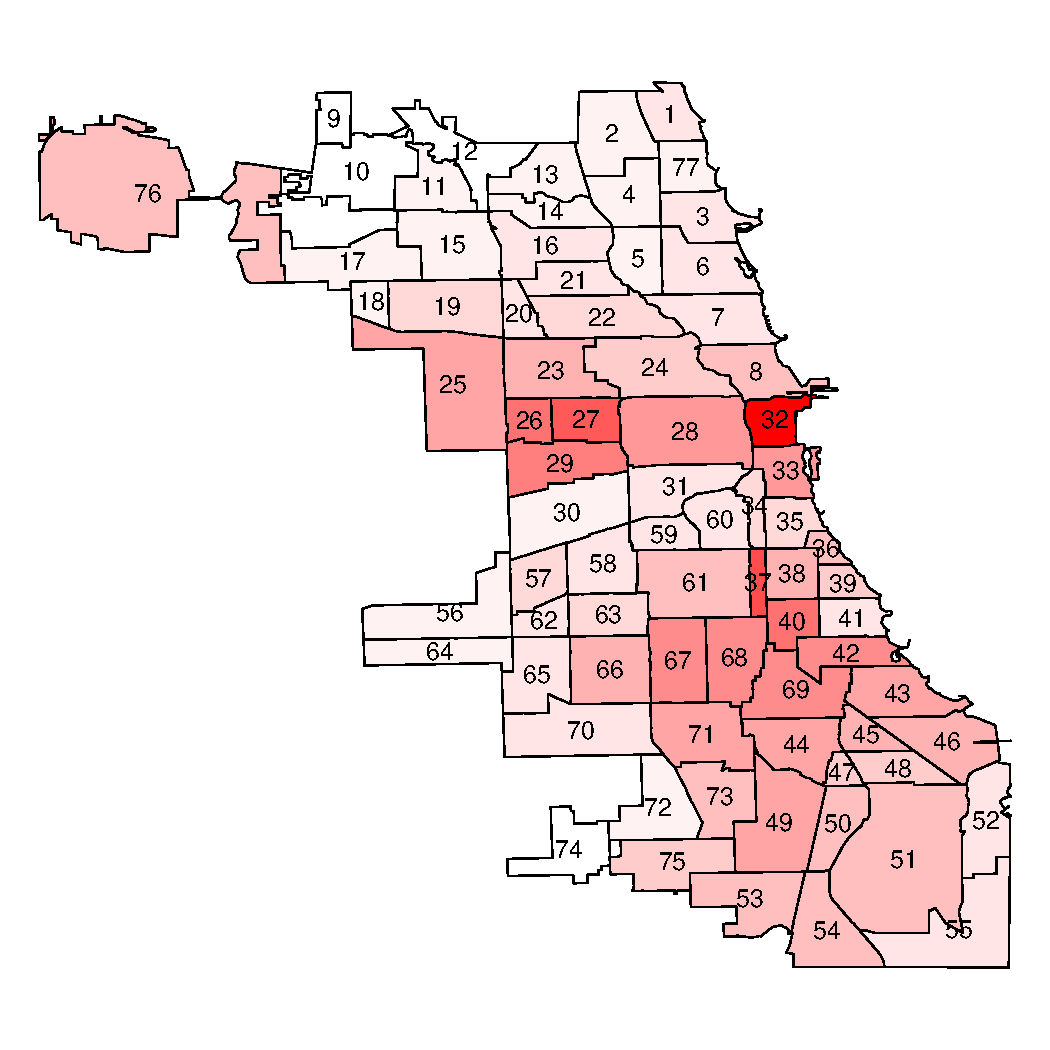
\includegraphics[width=0.5\textwidth]{fig/crime-ca.pdf}
\caption{Crime rate of Chicago by community areas. The community area \#32 is Chicago downtown, which has the highest crime rate.}
\label{fig:crime-ca}
\end{figure}


In this paper we study the crime rate inference problem. More specifically, we estimate the crime rate of some regions given the information of all the other regions. Without loss of generality, we assume there is one community area $t$ with crime rate $y_t$ missing, and we use the crime rate of all the other regions $\{y_i \} \backslash y_t$ to infer this missing value. Our problem is mathematically formalized as follows
\begin{equation}
\hat{y_t} = f( \{y_i\} \backslash y_t, X),
\end{equation}
where  $X$ refers to observed extra information of  all those community areas.




\smallskip
We consider two  types of features $X$ for inference: \vspace{-1mm}
\begin{itemize}[leftmargin=*]
\item Nodal feature. Nodal features describe the characteristics of the focal region. Such features include demographic information and Point-of-Interest (POI) distribution. Demographics are frequently used in literature, but POI is a newer type of big data, which we find significantly improve the crime inference accuracy.
\item Edge feature: (1) Geographical influence. Geographical influence considers the crime rate of the nearby locations.  This feature has been extensively used in
literature as well. To estimate the focal region, the
crime rate of nearby regions are weighted according
to spatial distances. (2) Hyperlink by taxi flow. Locations are connected through the frequent trips made by humans, which can be considered as the hyperlinks in space. This type of feature has never been studied in literature. We propose to use taxi trips to construct the social flow. Our hypothesis is that two regions that are more strongly connected through social flow will influence each other's crime rate.
\end{itemize}

In the following sections, we first discuss the inference models based on these three types of features in Section~\ref{sec:model} and then discuss how to construct these features using the real-world data in Section~\ref{sec:feature}.








\section{Inference Model}
\label{sec:model}


\subsection{Linear Regression}



The most straightforward prediction model is the linear regression. This model assumes the error terms follow a Gaussian distribution $\epsilon \sim \mathcal{N}(0, \sigma^2)$.


Equation~\ref{eq:lrm} gives the linear regression formulation of our problem.
\begin{equation}
\label{eq:lrm}
\vec{y} = \vec{\alpha}^T \vec{x} + \beta^f W^f \vec{y} + \beta^g W^g \vec{y} + \vec{\epsilon},
\end{equation}
where $\vec{x}$ represents the nodal features, including demographics and POI distribution, $W^f$ is the flow matrix of taxi flow, and $W^g$ is the spatial matrix representing the geographical adjacency. On the right-hand side, $\epsilon$ is the only stochastic variable, and all other terms are fixed observation values. Therefore, we incorporate all the fixed observations into one term $X$, and we get the standard regression problem
\[
E(y) = X w + \epsilon.
\]





\subsection{Negative Binomial Regression}


In our problem, we aim to infer the crime rate, which is guaranteed to be a non-negative integer. However, linear regression does not ensure this property. 
\emph{Poisson regression} is another form of regression, more appropriate for count data than linear regression \cite{GMS95}\cite{Lamb92}. With shortened notation $X$, the Poisson regression model has the exponential function as link function
\begin{equation}
\label{eq:prm}
E(y) = e^{X w}.
\end{equation}
This comes from the assumption that $y$ follows Poisson distribution with mean $\lambda $. Additionally, the mean $\lambda$ is determined by observed independent variables $X$, with the link function $\lambda = e^{Xw}$. Adding all together, the joint probability of $y$ is 
\begin{equation}
P(y|w) = \frac{e^{-e^{Xw}}(e^{Xw})^y}{y!}.
\end{equation}





However, Poisson regression enforces the mean and variance of dependent variable $y$ to be equal. This restriction leads to the ``over-dispersion'' issue for some real problems, that is the presence of larger variability in data set than the statistical model expected. To address this,  we use the Poisson-Gamma mixture model, which is also known as \emph{negative binomial regression}.  Negative binomial regression has been used in similar work~\cite{Osg00}.




Given that the crime rate $y$ follows Poisson distribution with mean $\lambda$, in order to allow for larger variance, $\lambda$ itself is a random variable having a Gamma distribution with shape $k=r$ and scale $\theta = \frac{1-p}{p}$.  The probability function of $y$ becomes
\begin{align}
P(y| r, p) & = \int_0^{\infty} P_{Poisson}(y|\lambda) \cdot P_{Gamma}(\lambda|r, p) d \lambda \nonumber \\ 
%		& = \int_0^{\infty} \frac{\lambda^y}{y!} e^{-\lambda} \cdot \lambda^{r-1} \frac{e^{-\lambda(1-p)/p}}{(\frac{p}{1-p})^y \Gamma(r)} d\lambda  \nonumber \\
		& = \frac{\Gamma(r+y)}{y! \Gamma(r)} p^k (1-p)^y
\end{align}
This is exactly the probability density function of negative binomial distribution.


In negative binomial regression, the link function is
\begin{equation}
E(y) = e^{X w + \epsilon}.
\end{equation}
The error term $e^\epsilon$ is the mixture prior, and we assume it follows Gamma distribution with shape parameter $k=\frac{1}{\theta}$, so that it has mean $E(e^\epsilon) = k\theta = 1$ and variance $Var(e^\epsilon) = k\theta^2 = \theta$. This setting ensures the $E(y) = e^{Xw} \cdot e^\epsilon = e^{Xw}$.

